\section{Iteración 2}
\label{sec:iteracion_2}

Después de que finalizó la primera iteración y ya que todas las pruebas pasaron exitosamente, se continúa con la segunda iteración.


\subsection{Iteration Planning Meeting}
\label{sub:iteration2_planning_meeting}


Al igual que la primera iteración, las fases de exploración y planeación se realizan al mismo tiempo, en el sentido que no es necesario repartir las tareas resultantes de la exploración, por lo tanto al mismo tiempo en que se determinan las tareas se puede realizar la estimación de las mismas.

  \subsubsection{Exploración y Planeación}
  \label{subs:iteration2_exploracion_planeacion}

  Para la segunda iteración se toman en cuenta todas las historias de usuario restantes, y de acuerdo al criterio de escoger las siguientes historias más relevantes y de mayor valor para el producto, se escogió la historia de usuario #4.\\

  Como parte de la fase de Exploración se toma la historia de usuario #4 y la dividimos en las Tareas de Ingeniería, las cuales serán trabajadas en la fase de la Implementación.

  En la siguente tabla se especificaran las tareas correspondientes a la historia de usuario #4 \ref{tab:us04_tasks}. \\

  \subsection{Tareas del US04}
  \label{sub:us04_tasks}

    \begin{table}[H]
  \begin{center}
    \begin{tabularx}{\textwidth}{ c  X  C{2.3cm} }
      \toprule
        \textbf{Código} &
        \multicolumn{1}{c}{\textbf{Tarea}} &
        \textbf{Estimación [dias]}\\

      \midrule
        T011
        &
        Crear un archivo shapefile con información inicial de lugares principales dentro el campus de la UMSS.
        &
        2 \\

      \addlinespace
        T012
        &
        Preparar la base de datos para manejar información geográfica de rutas.
        &
        1 \\
      %
      % \addlinespace
      %   T013
      %   &
      %   Investigar e instalar una herramienta que permita usar un servicio de mapas.
      %   &
      %   1 \\

      % \addlinespace
      %   T014
      %   &
      %   El usuario puede ver un mapa usando un servicio del campus de la UMSS.
      %   &
      %   0.5 \\

      % \addlinespace
      %   T015
      %   &
      %   El usuario puede ver un marcador sobre el lugar.
      %   &
      %   0.5 \\
      %
      % \addlinespace
      %   T016
      %   &
      %   El marcador tiene información básica del lugar, nombre, piso.
      %   &
      %   0.5 \\

      \addlinespace
        T017
        &
        El usuario puede ver un marcador mostrando el lugar actual donde se encuentra (el usuario).
        &
        0.5 \\

      \addlinespace
        T018
        &
        Desarrollar un módulo que encuentra la ruta más corta usando la base de datos con información geográfica ruteable de T012.
        &
        2 \\

      \addlinespace
        T019
        &
        El usuario puede ver una línea roja que une el marcador de la posición del usuario con el marcador del lugar.
        &
        1 \\

      % \addlinespace
      %   TS003
      %   &
      %   Crear pruebas de funcionalidad del US04.
      %   &
      %   1 \\

      \addlinespace
      \midrule
        & \multicolumn{1}{R{7cm}}{\textbf{Total: }}
        & 10 \\

      \bottomrule
    \end{tabularx}
    \caption{Tareas del US04}
    \label{tab:us04_tasks}
  \end{center}
\end{table}


  \subsection{Calendario de Entregas}
  \label{subs:schedule_2}

    % \begin{table}[!ht]
%
% \end{table}
\begin{table}[H]

  \begin{center}

\begin{ganttchart}[
  canvas/.append style={fill=none, draw=black!5, line width=.75pt},
  hgrid style/.style={draw=black!5, line width=.75pt},
  vgrid={*1{draw=black!5, line width=.75pt}},
  %today=0,
  % today label=Semana 3,
  today rule/.style={
    draw=black!64,
    dash pattern=on 3.5pt off 4.5pt,
    line width=1.5pt
  },
  today label font=\small\bfseries,
  title/.style={draw=none, fill=none},
  title label font=\bfseries\footnotesize,
  title label node/.append style={below=7pt},
  include title in canvas=false,
  bar label font=\mdseries\small\color{black!70},
  bar label node/.append style={left=2cm},
  bar/.append style={draw=none, fill=black!63},
  bar incomplete/.append style={fill=barblue},
  bar progress label font=\mdseries\footnotesize\color{black!70},
  group incomplete/.append style={fill=groupblue},
    group left shift=0,
    group right shift=0,
    group height=.5,
    group peaks tip position=0,
    group label node/.append style={left=.6cm},
    group progress label font=\bfseries\small,
    link/.style={-latex, line width=1.5pt, linkred},
    link label font=\scriptsize\bfseries,
    link label node/.append style={below left=-2pt and 0pt},
  ]{1}{12}
  \gantttitle{Calendario de Entregasde de la Iteración 2}{7} \\[grid]
  \gantttitle{Semana 1}{7}
  \gantttitle{Semana 2}{7} \\
  % \gantttitle{Noviembre}{4} \\
  \gantttitle[title label node/.append style={below left=7pt and -3pt}]{D\'ia:\quad15}{0}
  \gantttitlelist{16,...,30}{1} \\
  % \ganttgroup[progress=0]{Historias de Usuario}{1}{8} \\
  \ganttbar[
    progress=0,
    name=bar1
  ]{\textbf{User Story 04}}{1}{12} \\
  % \ganttbar[
  %   progress=0,
  %   name=bar2
  % ]{\textbf{User Story 03}}{10}{12} \\
  % \ganttbar[
  %   progress=0,
  %   name=bar3
  % ]{\textbf{Iteración 3}}{5}{6} \\
  % \ganttbar[
  %   progress=0,
  %   name=bar4
  % ]{\textbf{Iteración 4}}{7}{8} \\
  % \ganttbar[
  %   progress=100,
  %   name=bar5
  % ]{\textbf{Actividad 5}}{5}{7} \\
  % \ganttbar[
  %   progress=80,
  % ]{\textbf{Actividad 6}}{8}{8} \\
  % \ganttbar[
  %   progress=49,
  % ]{\textbf{Actividad 7}}{9}{11} \\
  % \ganttmilestone{Hito 1}{11}{11}  \\
  % \ganttmilestone{Hito 2}{12}{12} \\
  %

  % \ganttmilestone{Q6 report}{24}{24} \\
  % \ganttmilestone{M1: Project finished}{8}{8}

  % \ganttlink[link type=f-s]{bar1}{bar2}
  % \ganttlink[link type=f-s]{bar2}{bar3}
  % \ganttlink[link type=f-s]{bar3}{bar4}

\end{ganttchart}

\caption{Calendario de Entregas de la Iteración 2}
\label{tab:calendario_entregas_iteracion_2}

\end{center}
\end{table}



\subsection{Implementación}
\label{sub:implementacion_iteracion_1}

Durante esta fase es donde se implementaran las tareas especificadas en la tabla \ref{tab:us04_tasks}.

\subsubsection{RF011}
\label{subs:RF011}

% Crear un archivo shapefile con la información geográfica de las rutas internas del campus de la UMSS

% Como ya se explico en \ref{sec:ruta_corta_umss}, esta tarea se llevo a cabo recabando la informacion geoespacial con un dispositivo GPS y exportando los datos resultantes a un archivo shapefile, el cual se puede apreciar en \ref{fig:shapefile_umss_v1}.

\subsubsection{RF012}
\label{subs:RF012}

% Preparar la base de datos para manejar información geográfica de rutas

% Para realizar esta tarea se procedió a instalar pgRouting, el resultado de esta tarea se puede apreciar en el manual de instalación ## \\
%
% Una vez configurada la base de datos se procede a cargar la misma con la informacion obtenida en RF011, para tal efecto es necesario primeramente crear una tabla que contendra los LINESTRING contenidos en el shapefile, esta operacion es similar a la realizada en la tarea - RF003 (\ref{sub:RF003}). Una vez que ya se tiene la tabla a la llamamos \emph{ways}, se necesita ejecutar un query propio de \emph{pgRouting} el cual tiene como objetivo analizar los datos geo-espaciales de la tabla y a\~nadirle una \emph{topologia}.
%
% Dentro lo que es la \emph{topologia geoespacial} existe una aplicacion que se lo conoce como \emph{topología de red}. La \emph{topología de red} representa las relaciones entre segmentos en una red lineal o una colección de segmentos de línea\cite{osgeo_journal_topology}.
% En un \emph{SIG} la topologia ayuda a mejorar el analisis de datos geo-espaciales, para resolver el problema de la ruta corta \emph{pgRouting} genera una \emph{topología de red} usando los datos que existen en la tabla \emph{ways}, es necesario ejecutar una instruccion, la que se muestra a continiacion y \emph{pgRouting} se encarga de llenar los datos que se pueden observar en la figura \ref{fig:postgres_ways}, las columnas \emph{source} y \emph{target} son populadas con el analisis topologico y en la figura \ref{fig:postgres_vertices}, se puede observar que la tabla \emph{ways\_vertices\_pgr} es creada enteramente en la ejecucion de la instruccion.
%
% \begin{verbatim}
%   select pgr_createTopology('ways', 0.00000001, 'geom', 'gid');
% \end{verbatim}
%
% \begin{figure}[H]
%   \begin{center}
%     \caption{Vista de la tabla \emph{ways} en la base de datos PostgreSQL.}
%     \label{fig:postgres_ways}
%     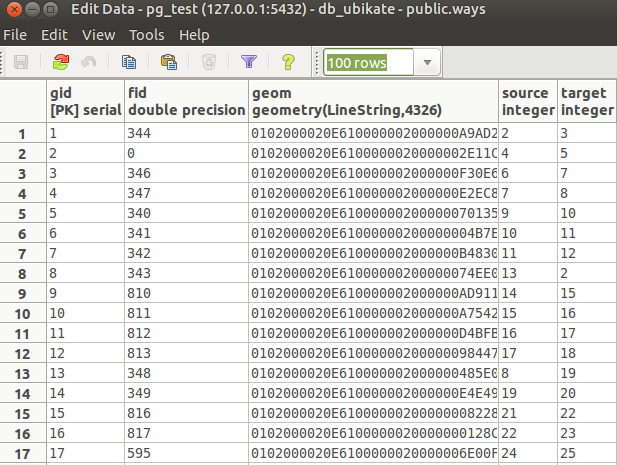
\includegraphics[width=1\textwidth]{iteration2/postgres_ways}
%     \caption*{Fuente: Elaboración propia}
%   \end{center}
% \end{figure}
%
% En la figura \ref{fig:postgres_ways} se puede apreciar que cada fila es una parte de la línea original obtenida por el dispositivo GPS y explisionada por QGIS, hay que notar que las columnas \emph{source} y \emph{target} hacen referencia a los nodos o vertices que la primera linea tiene en sus extremos, la primera linea o fila esta identificada por la columna \emph{gid}.\\
%
% En la siguiente figura \ref{fig:postgres_vertices} se observa la tabla \emph{ways\_vertices\_pgr} que contiene los vertices creados a partir del analisis de los datos en la tabla \emph{ways}.
%
% \begin{figure}[H]
%   \begin{center}
%     \caption{Vista de la tabla \emph{ways\_vertices\_pgr} en la base de datos PostgreSQL.}
%     \label{fig:postgres_vertices}
%     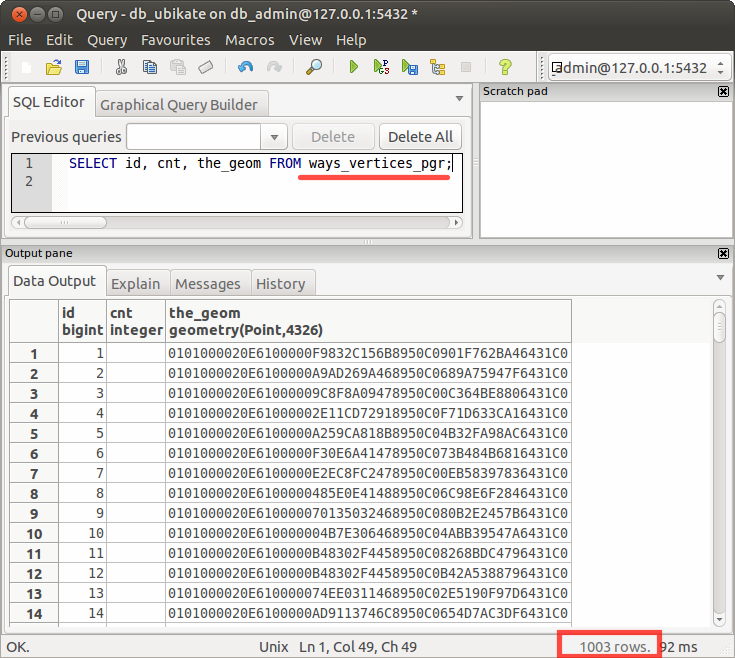
\includegraphics[width=1\textwidth]{iteration2/postgres_vertices}
%     \caption*{Fuente: Elaboración propia}
%   \end{center}
% \end{figure}
%
% Para entender los datos generados hay leer la informacion de las 2 tablas, por ejemplo en la primera  fila (gid 1) de la tabla \emph{ways}, se observa que el contenido de la columna \emph{source} es igual a \textbf{2} y \emph{target} es igual a \textbf{3}, eso quiere decir que los vertices del LINESTRING de la fila 1 son los vertices con \textbf{id} 2 y 3 respectivamente de la tabla \emph{ways\_vertices\_pgr}.\\
%
%
% Todo el conjunto de vertices y lineas de estas tablas se podria representar con una Matriz de adyacencias, explicada en \ref{sub:representacion_de_un_grafo}, y usada en la resolucion de la ruta mas corta, mas especificamente con el algoritmo de Dijkstra.

\subsubsection{RF013}
\label{subs:RF013}

% Investigar e instalar una herramienta que permita usar un servicio de mapas
% Durante la investigacion de esta tarea se encontro \emph{ember-leaflet}, una libreria o plugin que contiene las herramientas para poder cargar y usar un servicio de mapas.\\
%
% Para instalar esta libreria solo se necesita ejecutar el siguiente comando y posteriormente ya se puede empezar a utilizarla.\\
%
% \begin{verbatim}
%   $ ember install ember-leaflet
% \end{verbatim}
%
% El resultado de la investigacion puede apreciar en el marco teórico, en la sección que describe la librería, \emph{ember-leaflet}. \ref{sec:ember_js}

\subsubsection{RF014}
\label{subs:RF014}

% El usuario puede ver un mapa usando un servicio del campus de la UMSS

Para completar esta tarea se hizo uso de la herramienta \emph{ember-leaflet}, con la cual se puede desplegar un mapa en el browser y optimizada para dispositivos moviles.\\

\begin{verbatim}
  {{#leaflet-map lat=lat lng=lng zoom=zoom}}
    {{tile-layer
      url="http://{s}.tile.openstreetmap.fr/hot/{z}/{x}/{y}.png"
    }}
  {{/leaflet-map}}
\end{verbatim}

Con la anterior instrucción se accede al servicio de \emph{Open Street Maps}, de la cual obtenemos los datos necesarios para renderizar un mapa en el browser. Los atributos de \emph{lat} y \emph{lng} se acceden de la capa del controlador de la aplicacion, son la latitud y longitud respectivamente, la convinacion de ambos datos es la locacion donde se va a ubicar el renderizado del mapa.\\

% Esta librería es la nos ayudará a insertar fácilmente los marcadores que irán sobre los lugares o la líneas que mostraran la ruta más corta
%
% Como resultado de esta tarea se puede apreciar la siguiente figura,

\subsubsection{RF015}
\label{subs:RF015}
% El usuario puede ver un marcador sobre el lugar

Para completar esta tarea se continuó usando la librería \emph{ember-leaflet}, la cual permite que con la siguiente instrucción se despliegue un marcador sobre el mapa renderizado del API de \emph{Open Street Maps}.

\begin{verbatim}
  {{#marker-layer location=userLocation}} {{/marker-layer}}
\end{verbatim}

El resultado de la tarea se puede observar en la figura \ref{fig:baquita_place}.

\subsubsection{RF016}
\label{subs:RF016}
% marcador se  tiene información básica del lugar, nombre, piso

Para poder mostrar la informacion del lugar sobre el marcador creado en RF015 se hizo uso de la librería \emph{ember-leaflet}, al igual que dicha tarea, solo se necesito de una instruccion para poder desplegar la informacion necesaria.

\begin{verbatim}
  {{#marker-layer location=location}}
    h3>{{model.name}}</h3>
    {{model.description}}
    <strong>telf:</strong> {{model.phone}}
    <strong>piso#</strong> {{model.level}}
  {{/marker-layer}}
\end{verbatim}

En la figura \ref{fig:baquita_place} se puede apreciar el marcador con la información desplegada del lugar ``Baquita''.

\begin{figure}[H]
  \begin{center}
    \caption{Tooltip con la información de un lugar.}
    \label{fig:baquita_place}
    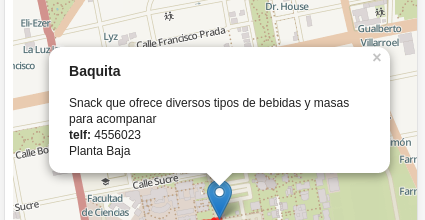
\includegraphics[width=1\textwidth]{iteration2/baquita_place}
    \caption*{Fuente: Elaboración propia.}
  \end{center}
\end{figure}


\subsubsection{RF017}
\label{subs:RF017}
% El usuario puede ver un marcador mostrando el lugar actual donde se encuentra (el usuario)

Para encontrar la locación del usuario se uso el API de geolocalización propio de HTML5, que en un smarthphone puede acceder y usar los recursos nativos de un smartphone, es necesaria la aceptacion del usuario mediante un mensaje que el navegador desplega, la locacion es encontrada mediante la triangulacion de Coordenadas por GPS (el mas exacto a la hora de encontrar la locacion del dispositvo), Wi-Fi, GSM o CDMA. Solo es necesaria la ejecucion de la siguente linea para ponder obetener la posición actual del usuario usando el API de geolocalización de HTML5.

\begin{verbatim}
  var coords = Geolocation.getCurrentPosition();
  var latitud = coords.latitude;
  var longitud = coords.longitude;
\end{verbatim}

La \emph{latitud} y \emph{longitud} obtenidas es fácilmente trasladado al mapa usando \emph{ember-leaflet} mediante un marcador, como se puede apreciar en la siguiente figura.

\begin{figure}[H]
  \begin{center}
    \caption{Tooltip con la latitud y longitud de la posición actual del usuario.}
    \label{fig:location_marker}
    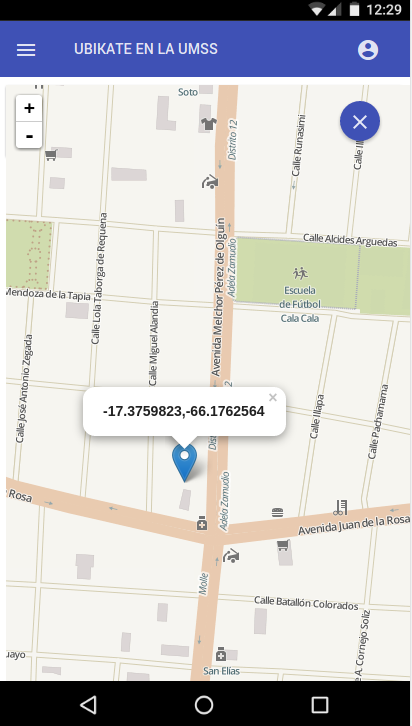
\includegraphics[width=0.5\textwidth]{iteration2/location_marker}
    \caption*{Fuente: Elaboración propia.}
  \end{center}
\end{figure}

\subsubsection{RF018}
\label{subs:RF018}
% Desarrollar un módulo que encuentra la ruta más corta usando la base de datos con información geográfica ruteable de RF012

Durante esta tarea se investigó la mejor forma de encontrar la ruta más corta y se llegó a la conclusión de usar la combinación de \emph{Postgres + Postgis + pgRouting}, esta investigación se puede apreciar en el marco teórico.\\

Para hallar la ruta más corta se necesita usar las características de la base de datos para poder analizar los datos geográficos almacenados en la Tarea RF012, como el análisis que se requiere hacer es caro osea el costo de procesador para realizar los calculos necesarios es elevado, lo mas recomendable es que este trabajo sea realizado en el backend de la aplicacion por la base de datos.\\

Tambien hay que tomar en cuenta que la tierra no es plana y las líneas que en un mapa parecen lineas rectas, realmente no son rectas, ya que el planeta Tierra es un \emph{esferoide oblato}\footnote{Un \emph{esferoide oblato} (o elipsoide oblato) es un elipsoide de revolución obtenido por rotación de una elipse alrededor de su eje más corto.} por lo que las lineas en apariencia rectas tienen la curvatura natural del planeta Tierra. En distancias largas esto tiene un gran impacto al manejar o utilizar mapas projectados, pero tambien es cierto que para una área pequeña como es el campus de la Universidad de San Simón este problema no tiene un gran impacto pero no está demás en tomar en cuenta esta característica del análisis de datos geoespaciales, como se explico en el capitulo \ref{cha:geolocalizacion}, para el presente proyecto se usara el proyeccion \emph{SRID 3857}.\\

Una vez que se tienen en cuanta estas variables es necesaria la resolucion del problema de la ruta más corta, \emph{pgRouting} tiene varios métodos implementados para el analisis de datos geo-espaciales en la resolucion de este problema, para el presente proyecto se usara el algoritmo de \emph{Dijkstra}, explicado en el capítulo \ref{cha:ruta_optima}.\\

Tomando en cuenta los conceptos aprendidos y las herramientas investigadas es que se desarrollo el modulo que encuentra la ruta mas corta.

% La siguiente SQL query está diseñado y explicado en la documentación de pgRouting {ref - link}, básicamente se necesita especificar el nodo inicio y el nodo destino y la base de datos se encarga de analizar la tabla creada en RF012, para que el algoritmo de Dijkstra funcione hay que darle un Costo a cada uno de los tramos pertenecientes a la Matriz, en este caso el costo será la longitud del tramo(st_length(geom) AS cost),  el costo de ir del punto A al punto B puede no ser la misma que de ir del punto B al punto A a pesar de ser una única línea, por ejemplo si la circulación fuera en un solo sentido  como en el caso de las rutas para automoviles, en este caso como es una ruta peatonal se simplifica un poco el problema, entonces como datos de entrada tenemos el punto donde se encuentra el usuario extraído por RF017 y el punto del lugar buscado extraído por RF0##, tomando en cuenta estos datos se armó el siguiente query,

% var raw = "SELECT seq, id1 AS node, id2 AS edge, cost " +
%             "FROM pgr_dijkstra('SELECT gid AS id, source::integer, target::integer, st_length(geom) AS cost " +
%             "                   FROM public.ways', " + targetId + ", " + sourceId + ", false, false);";

\subsubsection{RF019}
\label{subs:RF019}
% El usuario puede ver una línea roja que une el marcador de la posición del usuario con el marcador del lugar
Como resultado de la tarea RF018 se tiene un conjunto de datos en formato de latitud y longitud que conforman líneas, las cuales representan la ruta más corta, pero al final es solo un montón de números, útiles pero para el usuario esta información es difícil de procesar, el usuario necesita información que sea fácil de entender y no existe mejor herramienta disponible para esta tarea que mostrar la \emph{ruta} de forma visual, esto quiere decir que se necesita mostrar la ruta sobre un \emph{mapa}, en la aplicación se usará \emph{ember-leaflet} para desplegar el mapa ofrecido por los servicios de OpenStreetMaps y también para mostrar ruta más corta mediante una línea de color rojo.\\

Para resolver esta tarea se creó un servicio API usando ExpressJS, la cual se encarga obtener la información extraída de la base de datos y transformarla en un objeto JSON (GeoJSON), este objeto contiene la información geoespacial necesaria para ``dibujar'' la línea roja entre 2 puntos georeferenciados, uno de los cuales es el lugar al que se quiere llegar y el otro es la ubicación actual del usuario. \\

\begin{verbatim}
  ENV.APP.API_HOST + '/api/v1/ways/route/' + sourceData.id + '/' + targetData.id;

  GET /api/v1/ways/route/930/77 200 276.217 ms - 3911

  $ curl http://localhost:3000/api/v1/ways/route/930/77 | python -m json.tool                                                       [3:04:52]
  % Total    % Received % Xferd  Average Speed   Time    Time     Time  Current
                                 Dload  Upload   Total   Spent    Left  Speed
100  3911  100  3911    0     0   161k      0 --:--:-- --:--:-- --:--:--  166k
{
    "features": [
        {
            "geometry": {
                "coordinates": [
                    [
                        -66.1467397848201,
                        -17.3935321732846
                    ],
                    [
                        -66.1467190789842,
                        -17.3935294725234
                    ]
                ],
                "type": "LineString"
            },
            "type": "Feature"
        },

\end{verbatim}
% /api/v1/ways/route/

% Este objeto es representado en el mapa usando ember-leaflet con la siguiente instrucción,
%
% {{#geojson-layer geoJSON=currentGeoJSON color='red' }}
% {{/geojson-layer}}

Y se puede observar en el mapa una línea roja que representa la ruta más corta entre el punto donde se encuentra el usuario y el punto del lugar a buscar.

\begin{figure}[H]
  \begin{center}
    \caption{Ruta más corta dibujada con una línea roja.}
    \label{fig:short_way_place}
    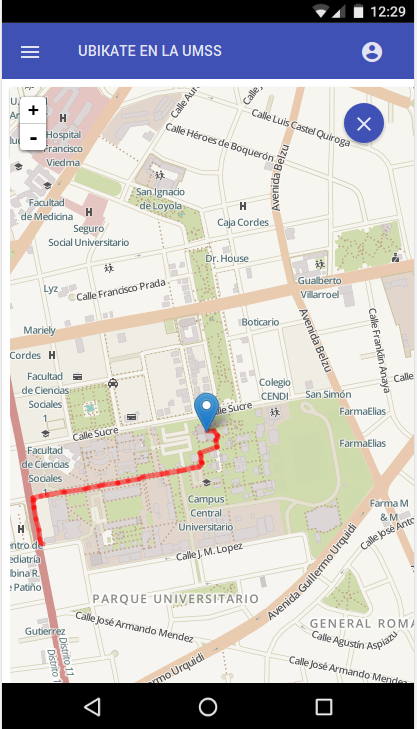
\includegraphics[width=0.5\textwidth]{iteration2/short_way_place}
    \caption*{Fuente: Elaboración propia.}
  \end{center}
\end{figure}

\subsubsection{TS004}
\label{subs:TS004}

Pruebas funcionales

\subsection{Registrar el Avance}
\label{sub:iteracion2_avance}

\subsection{Verificación}
\label{sub:iteracion2_verificacion}
